%!Tex root=../report.tex

\begin{figure*}[ht!]
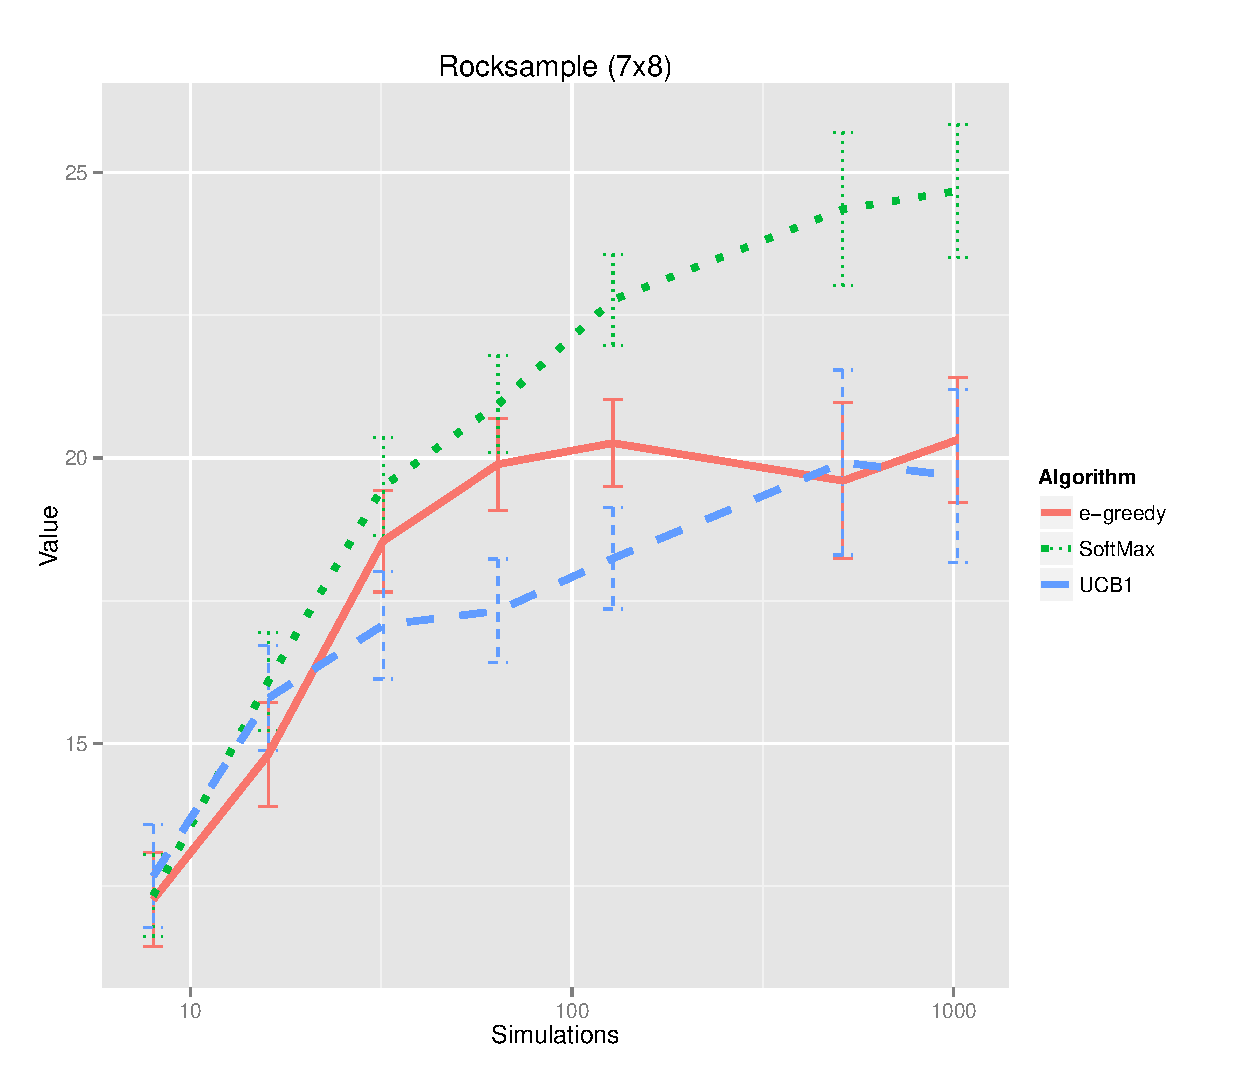
\includegraphics[width=.5\linewidth,height=.3\linewidth]{rocksample78.eps}
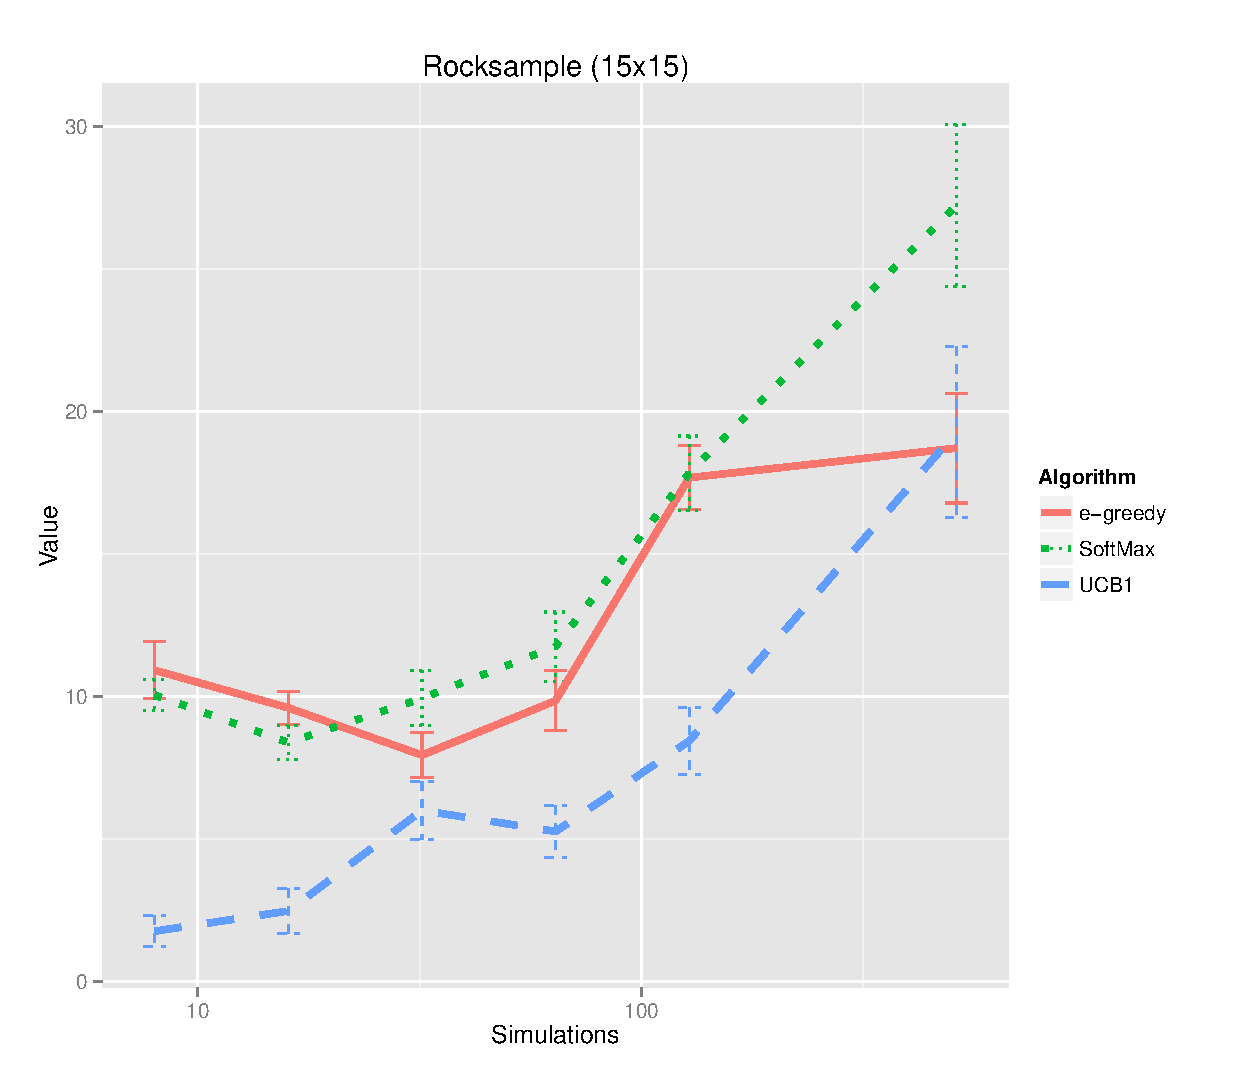
\includegraphics[width=.5\linewidth,height=.3\linewidth]{rocksample1515.eps}
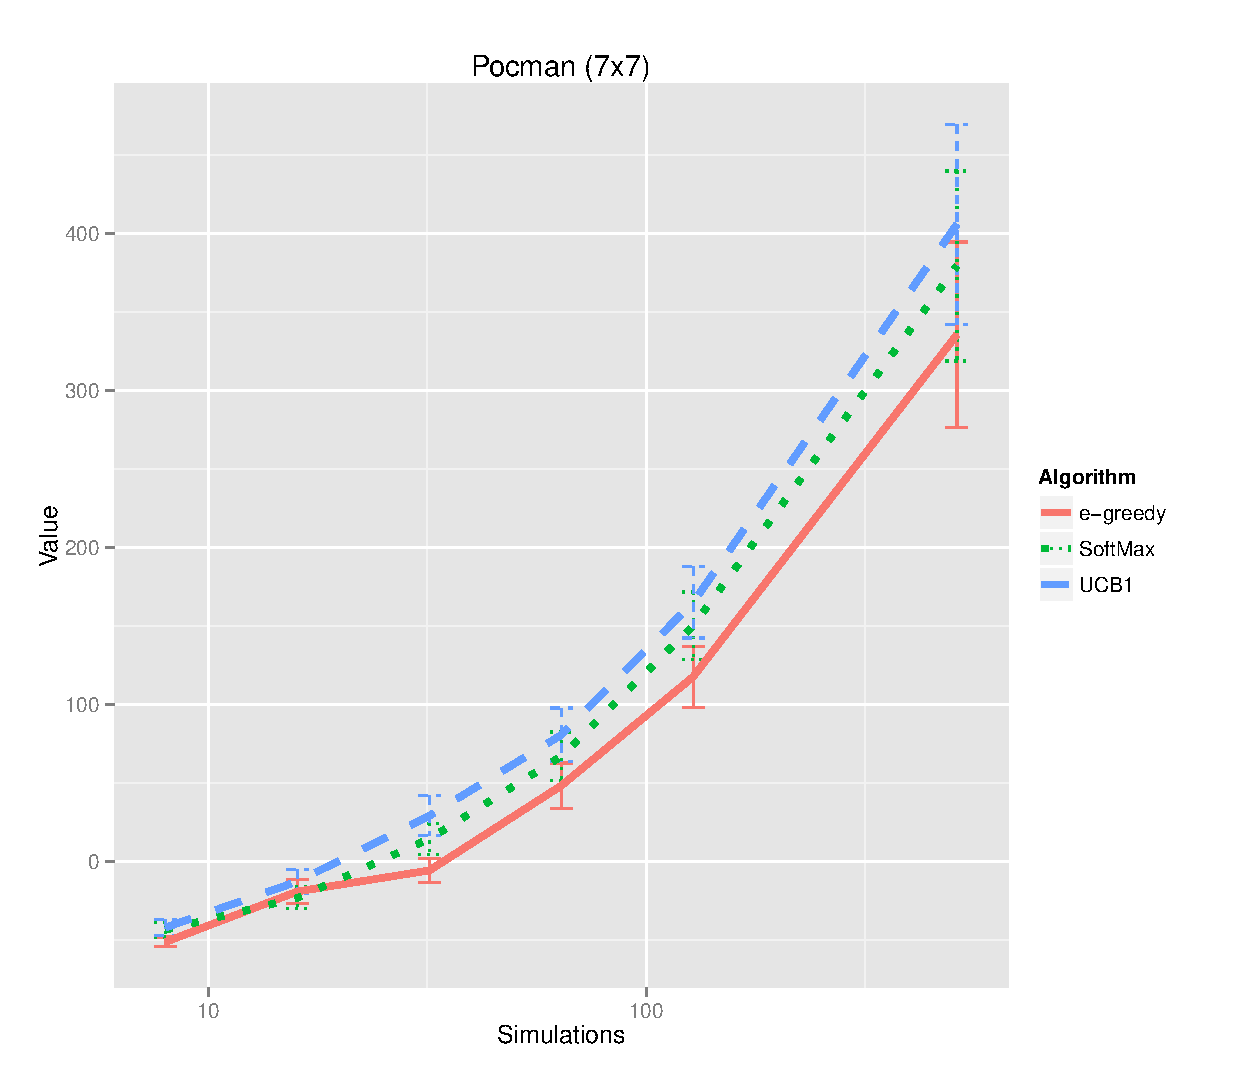
\includegraphics[width=.5\linewidth,height=.3\linewidth]{pocman77.eps}
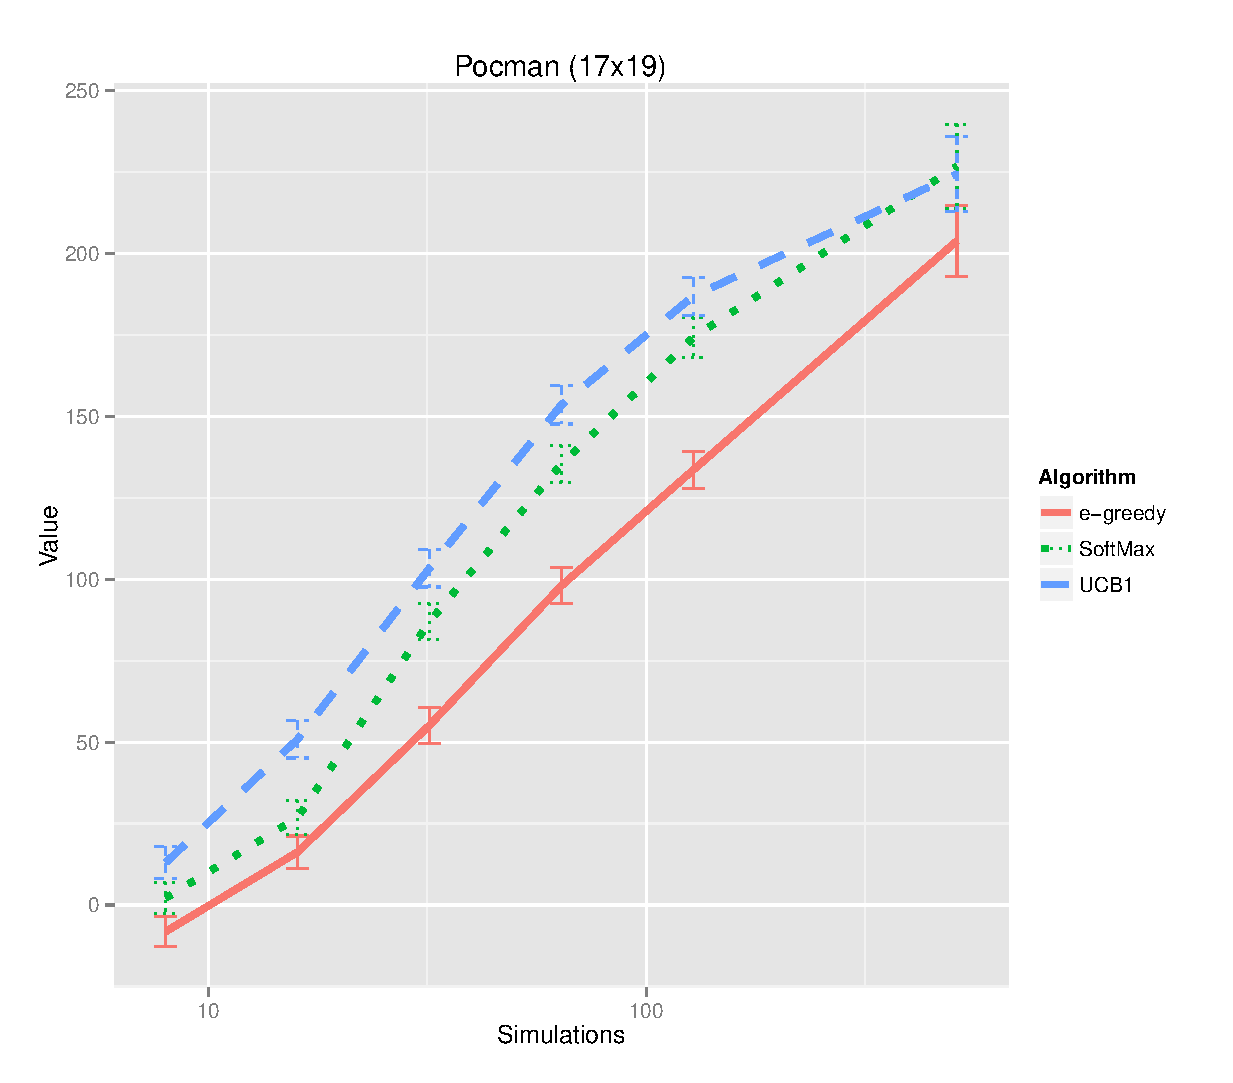
\includegraphics[width=.5\linewidth,height=.3\linewidth]{pocman1719.eps}
\caption{Comparison of UCB1, \soft and \egreedy on two \rock instances and two \poc instances. Note the log-scale on the x-axis, reflecting the increase in simulations. 95\% confidence intervals are indicated on each plot point.}
\label{fig:results1}
\end{figure*}

\section{Evaluation}
\label{sec:eval}
We conduct our analysis of the selected heuristics in three steps, investigating each of the initially studied heuristics separately. Furthermore, to better understand the reason for their relative performance, we propose and evaluate extensions for both \egreedy and \soft. Firstly, we seek to establish whether the default usage of UCB1 is justified on POMDP instances. To this end, we compare UCB1 with two commonly used general-purpose search heuristics: \soft and \egreedy on both the two instances of \rock and of \poc. The results are shown in \Cref{fig:results1}.


\subsection{Performance of UCB1}
As can be seen, performance varies substantially between \rock and \poc. In particular, all algorithms performed comparably on the \poc instances whereas larger gaps in performance were observed on the \rock instances. We identify two probable causes for this discrepancy, which both affect performance of the heuristics: firstly, the number of actions available at every step is much larger in \rock than in \poc (13 \vs 4). The impact of this difference becomes apparent when considering that each simulation recursively chooses an action up to 100 steps ahead. Whereas 256 simulation would suffice to cover all branches up to four steps ahead in \poc, it would only just suffice for two steps in \rock. The second cause lies with the presence of dynamic elements in \poc (ghosts), which may reduce the need to plan far ahead in taking actions.

Both these elements are reflected in the performance of UCB1. Whereas UCB1 is nearly consistently (and often substantially) outperformed on \rock, it achieves top performance (often shared with \soft) on \poc. UCB1 will initially explore all branches but is thereafter more keen to explore branches on which it previously found good performance. This is likely inefficient when many actions are present, as is the case on \rock, as the algorithm may too eagerly give up on an action when one subsequent path leads to poor results. On \poc, however, this strategy works to its advantage, allowing it to explore a few actions in great depth. 

\RS{1}{A greedy strategy is poorly equipped when many actions can be chosen.}

\subsection{Investigating $\varepsilon$-Greedy}
Roughly the inverse of UCB1's performance holds for \egreedy. In particular, \egreedy performs worse than \soft with a greater number of simulations and worse than both other heuristics in the case of a greater state space. This suggests that a constant degree of purely random exploration is inefficient. To evaluate this hypothesis, we propose \eroulette: a variation of \egreedy in which, with probability $\varepsilon$, the action is chosen through roulette wheel sampling based on the expected action value of each child. We compare this variation with \soft in \Cref{fig:results2}. As can be seen, performance improves only on \rock 7x8 and severely decreases on \poc. This suggests that a greater state-space necessitates a shift to increasingly greedy investigation of a few branches towards the end of each iteration. The improved performance on \rock 7x8 furthermore suggests that a greater number of simulations is more efficiently utilized by investigating multiple branches even towards the end of the search.

\RS{2}{Greater state-spaces necessitate increasingly greedy investigation.}

\begin{figure*}[ht!]
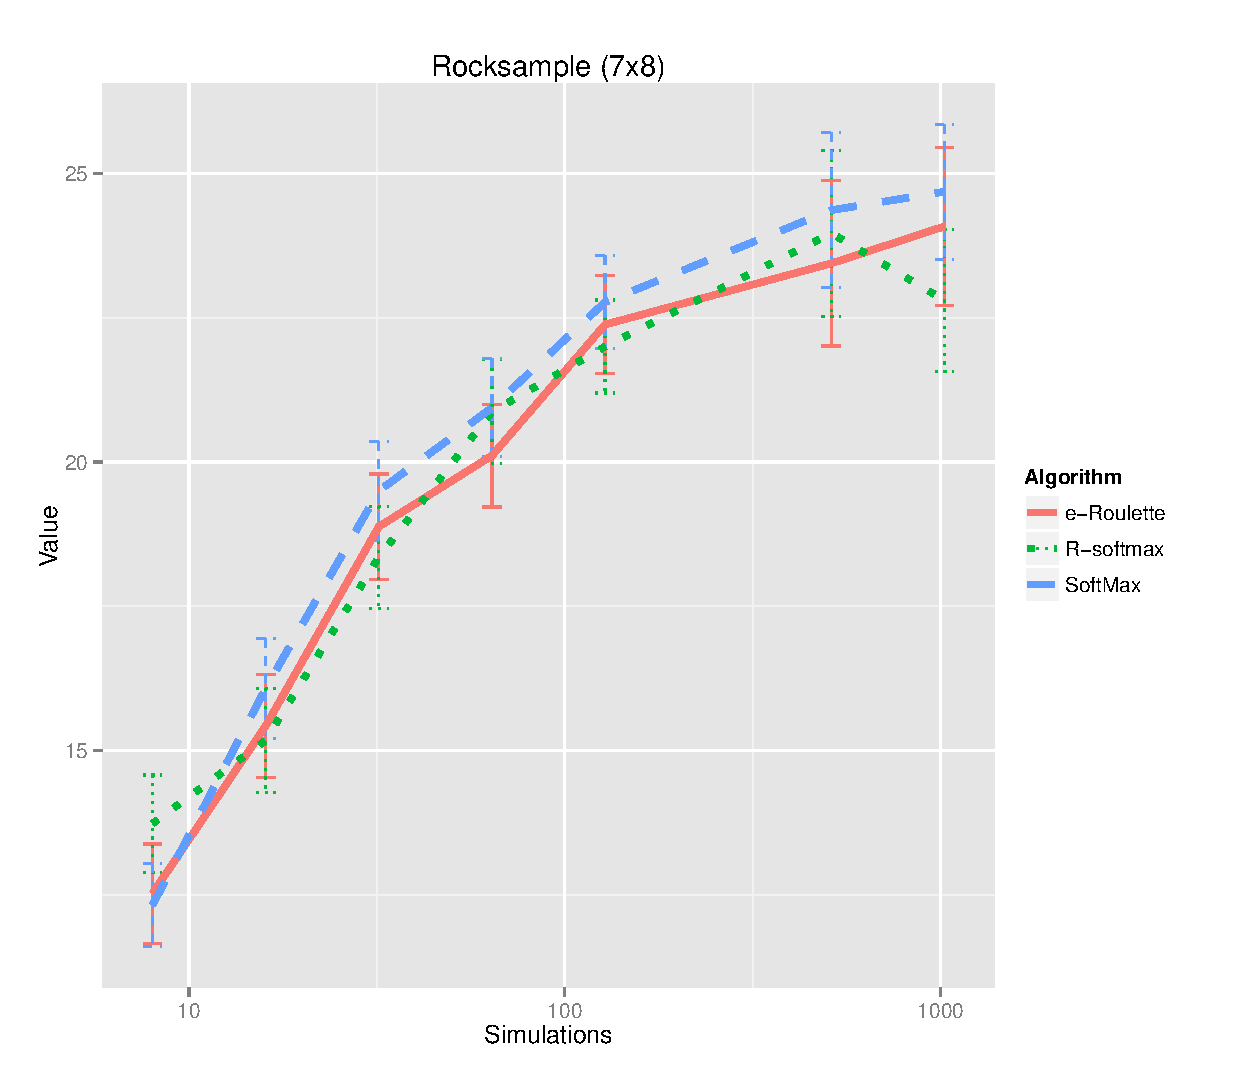
\includegraphics[width=.5\linewidth,height=.29\linewidth]{rocksample78b.eps}
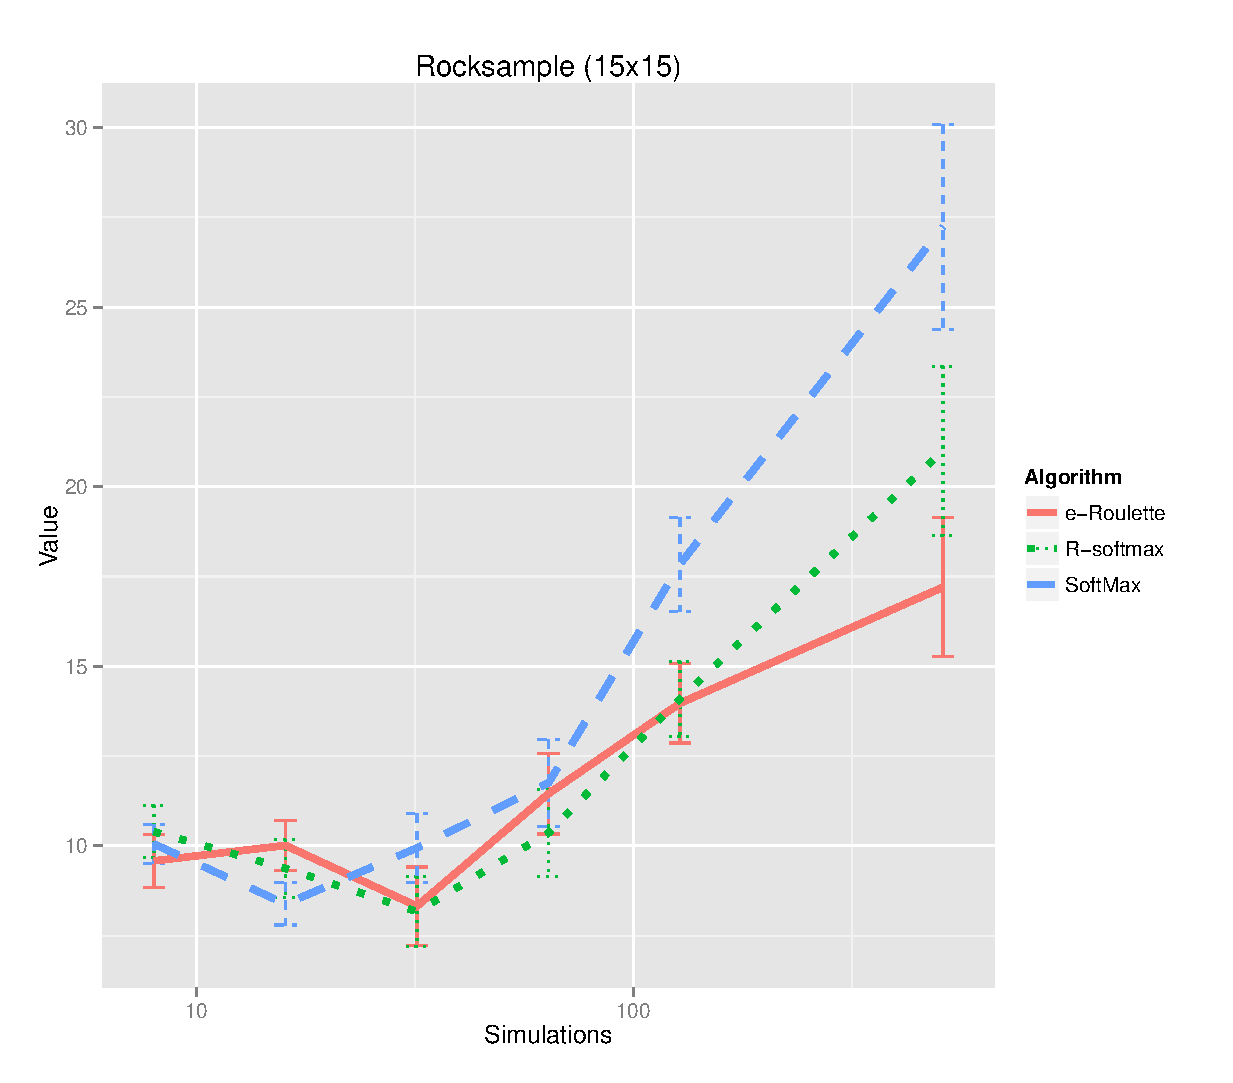
\includegraphics[width=.5\linewidth,height=.29\linewidth]{rocksample1515b.eps}
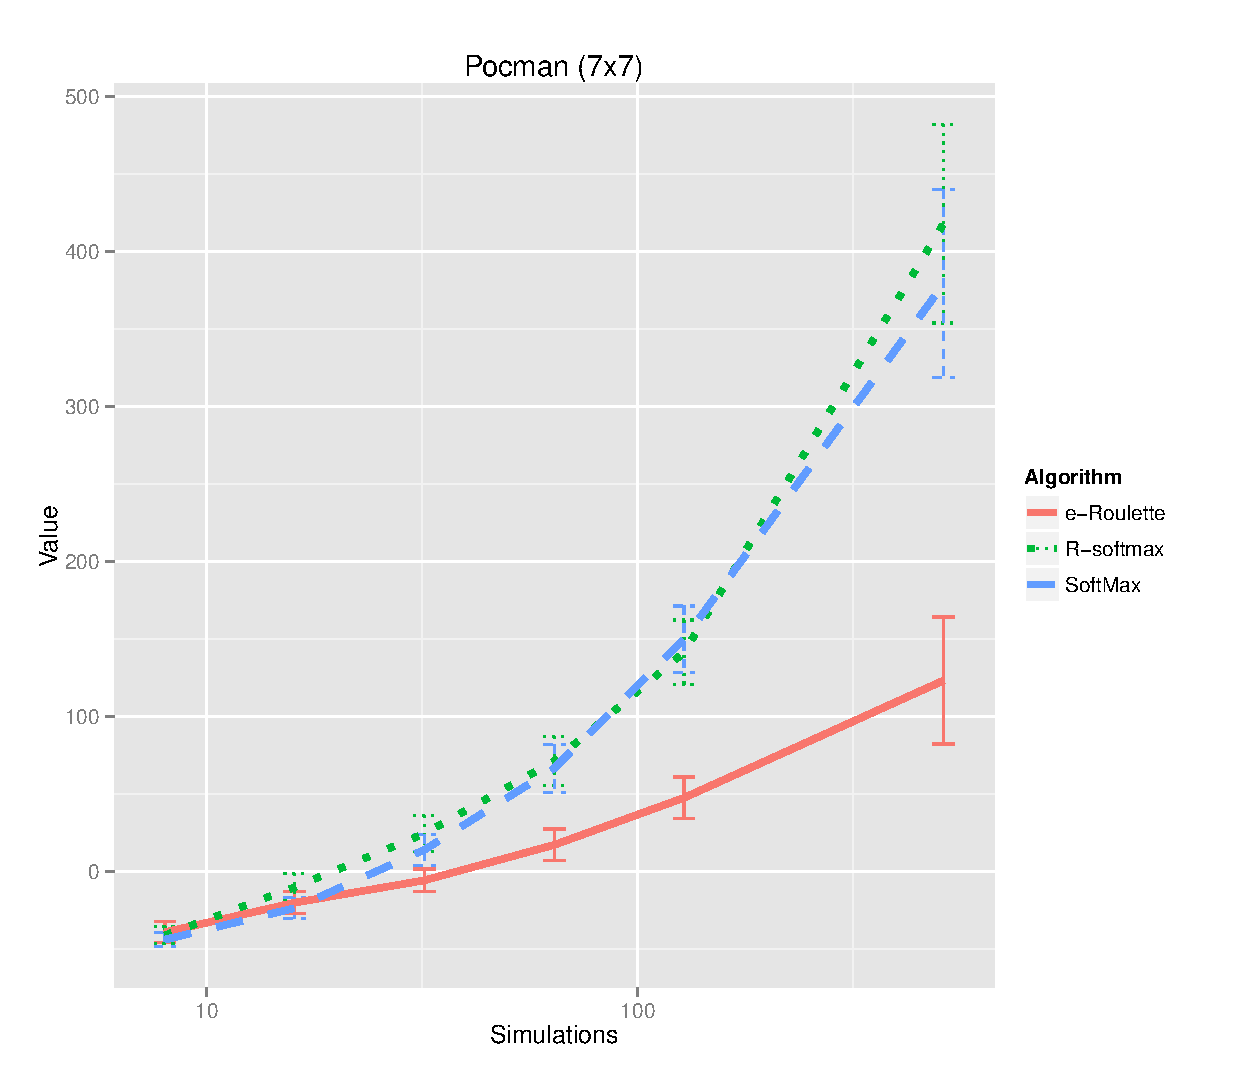
\includegraphics[width=.5\linewidth,height=.29\linewidth]{pocman77b.eps}
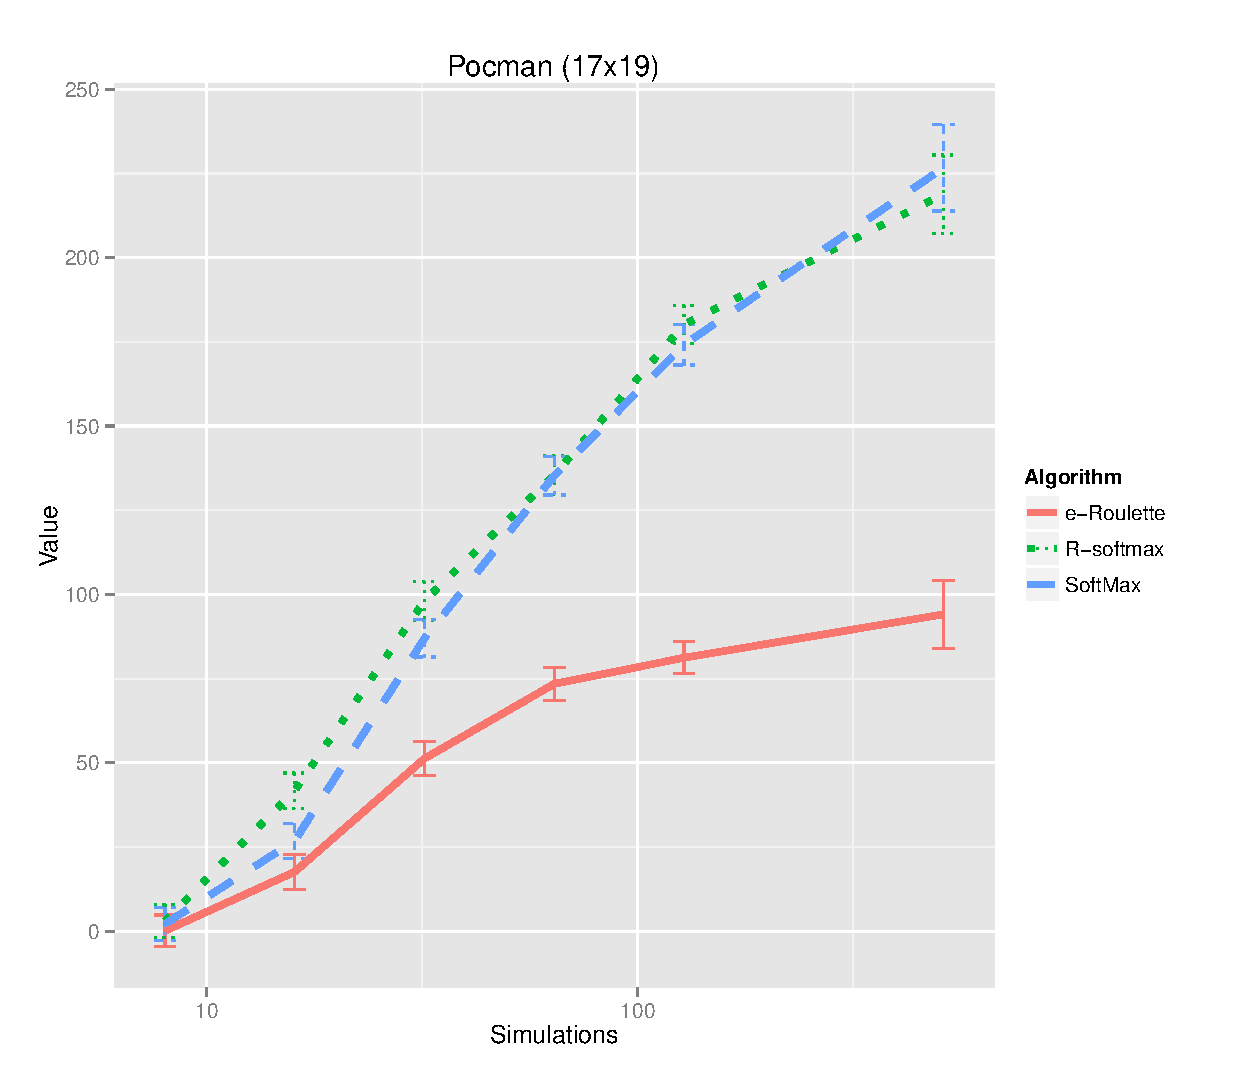
\includegraphics[width=.5\linewidth,height=.29\linewidth]{pocman1719b.eps}
\caption{Comparison of \soft to the two proposed variations: \rsoft and \eroulette, on the two \rock instances and the two \poc instances. Note the log-scale on the x-axis, reflecting the increase in simulations. 95\% confidence intervals are indicated on each plot point.}
\label{fig:results2}
\end{figure*}

\subsection{Investigating SoftMax}
In general, \soft performed best of the tested heuristics. \soft employs a temperature scheme in which the algorithm becomes progressively more greedy as the number of simulations increases. As such, it will initially visit all next actions with roughly equal likelihood and increasingly focus its search on promising branches. Its good performance has strong implications: it suggests that the tree structure can efficiently be exploited by using the relative amount of \emph{information} present at each node (what fraction of simulations were run) to suggest the amount of \emph{randomization} with which decisions should be made.

\RS{3}{\soft yields superior performance by connecting the degree of exploration to the total number of simulations.}

As was noted in \Cref{subsec:soft}, \soft suffers from the need to manually configure the $\tau$ parameter (both start and end value), as well as the rate of decrease of the temperature. We found that this parameter was very sensitive to the actual values of actions that were present in the problem, \eg for \poc a much higher initial value was needed than in \rock as different branches of the search tree yielded widely varying rewards. This strong dependency on the specified rewards for each action adds overhead to the application of this heuristic to a new domain.

We propose a variation to \soft named \rsoft. In this algorithm, we replace each reward with its \emph{rank} in the ordered list of rewards of all children of the current node under consideration. As such, the algorithm is substantially more robust to the absolute rewards chosen. We propose to initialize $\tau$ to the number of distinct actions present, as this will start the algorithm with a high degree of random exploration. We furthermore found that the resulting algorithm is fairly robust with respect to the final value of $\tau$ and suggest setting this to $1/4$. The results are shown in \Cref{fig:results2}. As can be seen, \rsoft almost consistently performs as well as \soft (which was hand-tuned on each instance), with the exception of \rock 15x15. Future work may further investigate extensions.

\RS{4}{\rsoft sacrifices little performance in favor of broader applicability to \soft by disregarding the values of rewards used in favor of their ordering.}
